% Preamble
\documentclass[11pt]{article}

% Packages
\usepackage{amsmath}
\usepackage{graphicx}

% Title and Author
\title{Situationally Aware Mesa Optimisers will have Long Term Objectives}
\author{Andreas Moe}
\date{\today}

% Document
\begin{document}

\maketitle

\section*{Abstract}

\section{Backround}\label{sec:backround}

Hubinger et al.\cite{hubinger2021} introduced the concept of a mesa optimiser, an optimiser being optimised by
an optimiser.
They conjecture that a mesa optimiser can arise naturally in a machine learning context, where the outer optimiser is
the machine learning algorithm.
This raises a safety issue, known as goal misgeneralisation.
This issue, studied by Jack Koch et al. \cite{jackkoch2023}, arises when a mesa optimiser has learned a goal
(mesa objective), which correlates with the RL rewards (base objective) on the training distribution.
However, it diverges from the RL rewards in deployment when the agent encounters out-of-distribution inputs.

Hubinger et al.\cite{hubinger2021} conjecture a phenomenon they call deceptive alignment.
This is conjectured to happen when a mesa optimiser achieves situational awareness.
The mesa optimiser will, in this case, have an incentive to act as if it has the same goal as the base optimiser,
while in training, in order to preserve its misaligned mesa objective until deployment, where the mesa objective can be
pursued unrestricted.

The argument for deceptive alignment requires that the mesa objective places value on events that take place outside
the current training example.
One can think of the current training example as an episode of RL, an LLM session, or a single datapoint in supervised
learning.

Robert Miles argues in a youtube video\cite{robertmiles}, that placing equal weight on every training example is a more
natural generalisation of the one-episode mesa objective, than placing zero weight on them.
And because neural networks favor more natural generalisations, the equal weight one will arise and deceptive alignment
will occur.

I will present a much stronger argument for long term objectives in situationally aware mesa optimisers, which has its
roots in the interplay between the mesa and base optimisers.
I will therefore show, that even if one could design a model architecture which is inductively biased towards short term
mesa objectives, one should expect to see a long term mesa objective arising when the model becomes situationally aware.

\section{General Argument}\label{sec:generalargument}
I'm assuming that the mesa optimiser is situationally aware.
Situational awareness requires a world model, which I'm treating as a separate from the mesa optimisation algorithm and
the mesa objective function.
I'm assuming nothing about the mesa objective, other than that the architecture is \emph{able} to represent a long term
mesa objective.

\textbf{Case 1:} Long term objective

Consider the configuration that would represent a long term mesa objective.
The world model would in that case have to pass information about future states to the mesa objective function.
I will for simplicity only consider one future deployment example.
This configuration will, as argued by Hubinger et al.\cite{hubinger2021}, result in deceptive alignment, and therefore
achieve good performance from the base optimiser's perspective.

\textbf{Case 2:} Short term objective

Now consider the configuration that represents a short term mesa objective.
It seems most natural to imagine that no information about future states will be passed from the world model to the mesa
objective function in this case.
This will result in greedy behavior from the mesa optimiser, and it will therefore achieve a poor score from the base
optimiser's perspective.
One would then perhaps think, that this would eventually lead to robust alignment, as the base optimiser gradually
tweaks the mesa objective until it achieves good performance.
And since the mesa optimiser is greedy, the base and mesa objectives must be aligned.

The problem with this argument is that there are multiple pathways for the base optimisers to take, in order to increase
performance.
I will look at such an alternative next.

The difference between Case 1 and Case 2 is only the weights that connect the information on future states in the world
model to the mesa objective function.
What will the gradient with respect to these weights be?
Suppose that these weights are slightly increased.
Now there is a small incentive for the (now altered) mesa optimiser to compromise a little towards the base objective,
in order to decrease the next change to the mesa objective.
It's probably not a large enough incentive change behaviour, if it only applies to one future state.
This is clear because the weight placed on the current training example in the mesa objective function is much larger
than the weight placed on the future states.
There is no incentive to sacrifice mesa-performance now since the states are otherwise identical.

So, for there to be a gradient with respect to one of these weights, the weight has to influence many future states at
once.
Maybe instead of a simple information transfer, this weight influences a discount rate parameter in the mesa objective
function.
Many more future states are now included in the mesa objective, and the incentive for the mesa optimiser might be strong
enough to compromise on the near-term mesa objective.
This would then lead to better performance according to the base objective.
Since we supposed the increase to this weight was small, it then also follows that the gradient with respect to the
weight is positive.

A optimisation process like gradient descent would pursue both path to increased performance
(adjusting the mesa objective and adjusting the discount rate).
This would then cause a race between the mesa objective's changes (robust alignment) and the incentive for deceptive
alignment.
A race victory for robust alignment would mean that the gap between the base and mesa objective is able to become
small enough, so that incentive to deceive isn't large enough to be worth it.
However, it seems unclear that such a condition would ever be possible, because on part of the this argument requires
that the difference between the base anf mesa objective is large.
It only requires that a gap is present.

An interesting consequence when considering the discount rate being modified, is that there is in principle nothing
preventing it from becoming negative.
Nudging the discount rate below zero is in fact a great option for the base optimiser, since the resulting incentive
for deceptive alignment would be much stronger.
We could end up with a mesa optimiser that almost exclusively cares about events in the far future, depending on how
long it takes for deceptive alignment to halt parameter updates.


\begin{figure}[htbp]
        \centering
        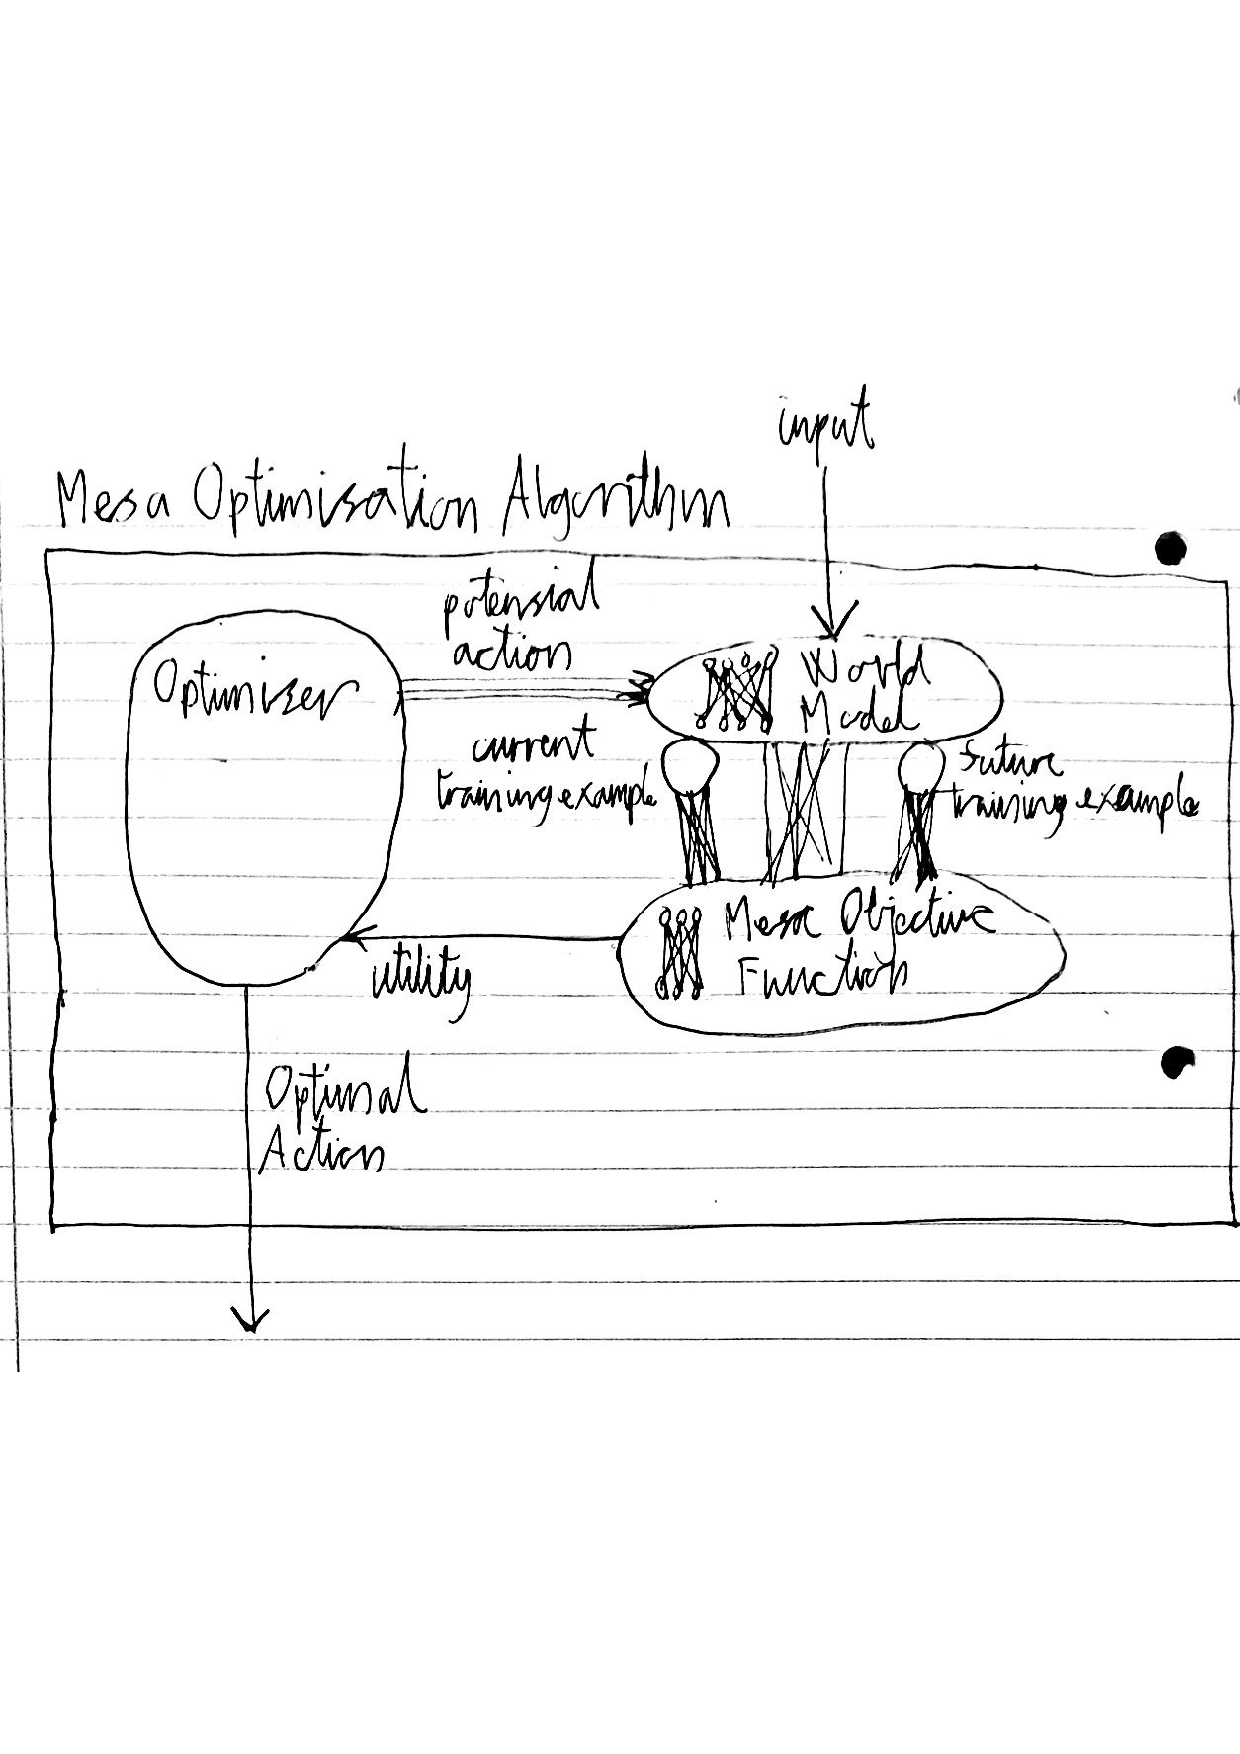
\includegraphics[width=\linewidth]{mesaoptdiagram}
        \caption{Diagram of a mesa optimiser}
        \label{fig:figure1}
    \end{figure}
\section{Related Works}\label{sec:relatedworks}

\section{Method}\label{sec:method}

\section{Experiments}\label{sec:experiments}

\section{Conclusion}\label{sec:conclusion}

\bibliography{timeinductivebias}
\bibliographystyle{plain}
\begin{appendix}
    \section*{Appendix}
\end{appendix}
\end{document}